\documentclass[11pt]{article}
\usepackage{amsmath, amsthm, amssymb}
\DeclareMathOperator{\Tr}{Tr}
\usepackage{amsfonts}
\usepackage{amssymb,amscd}
\usepackage{array}
\usepackage{indentfirst}
\usepackage{graphicx}
\usepackage{color}
\usepackage{float}
\usepackage{url}
\usepackage{bm}
\usepackage[super]{natbib}
\usepackage{braket}
\usepackage{enumerate}
\usepackage{caption}
\usepackage[font={footnotesize}]{subcaption}
\usepackage[normalem]{ulem}
\usepackage[left=1.25in,top=1.5in,bottom=1in,right=1.25in, nohead]{geometry}
\usepackage[space]{grffile}
\usepackage{multirow}
\usepackage{longtable}
\usepackage{hyperref}
\usepackage{booktabs}

%\usepackage[T1]{fontenc}
%\usepackage{garamondx}
%\usepackage[garamondx,cmbraces]{newtxmath}

%\usepackage[urw-garamond]{mathdesign}
\usepackage[T1]{fontenc}

\def\RR{{\mathbb R}}
\def\CC{{\mathbb C}}
\def\NN{{\mathbb N}}
\def\ZZ{{\mathbb Z}}
\def\QQ{{\mathbb Q}}
\def\H{{\mathcal H}}


% Different font in captions
\newcommand{\captionfonts}{\normalsize}

\makeatletter  % Allow the use of @ in command names
\long\def\@makecaption#1#2{%
  \vskip\abovecaptionskip
  \sbox\@tempboxa{{\captionfonts #1: #2}}%
  \ifdim \wd\@tempboxa >\hsize
    {\captionfonts #1: #2\par}
  \else
    \hbox to\hsize{\hfil\box\@tempboxa\hfil}%
  \fi
  \vskip\belowcaptionskip}
\makeatother   % Cancel the effect of \makeatletter

\newtheorem{theorem}{Theorem}[section]
\newtheorem{corollary}[theorem]{Corollary}
\newtheorem{proposition}[theorem]{Proposition}
\newtheorem{lemma}[theorem]{Lemma}

\makeatletter
\newsavebox\myboxA
\newsavebox\myboxB
\newlength\mylenA

\newcommand{\exedout}{%
  \rule{0.8\textwidth}{0.5\textwidth}%
}
\newcommand*\xoverline[2][0.75]{%
    \sbox{\myboxA}{$\m@th#2$}%
    \setbox\myboxB\null% Phantom box
    \ht\myboxB=\ht\myboxA%
    \dp\myboxB=\dp\myboxA%
    \wd\myboxB=#1\wd\myboxA% Scale phantom
    \sbox\myboxB{$\m@th\overline{\copy\myboxB}$}%  Overlined phantom
    \setlength\mylenA{\the\wd\myboxA}%   calc width diff
    \addtolength\mylenA{-\the\wd\myboxB}%
    \ifdim\wd\myboxB<\wd\myboxA%
       \rlap{\hskip 0.5\mylenA\usebox\myboxB}{\usebox\myboxA}%
    \else
        \hskip -0.5\mylenA\rlap{\usebox\myboxA}{\hskip 0.5\mylenA\usebox\myboxB}%
    \fi}

\newcommand{\verbatimfont}[1]{\renewcommand{\verbatim@font}{\ttfamily#1}}

\makeatother

\setlength{\intextsep}{10pt plus 2pt minus 2pt}
\title{Ward Character Sentiment Analysis}
\author{Aidan Klobuchar}
\date{}
\begin{document}
\maketitle
\section{Introduction}
\noindent
Ward is the wonderful fourth, in progress, web serial by the author Wildbow. It's a tale of superpowers, post-apocalyptic rebuilding, mysterious machinations, and how all of this relates to trauma and second chances. But more importantly, it is a LARGE collection of text, primarily told experienced through a first person perspective. This makes it an enticing dataset for messing around with some NLP. NLP, short for natural language processing, is a very popular, useful, and well-trodden area of machine learning and data science, specializing in the automatic analysis, summarization, tagging, etc. of human created text. One task that can be accomplished using NLP is known as \emph{sentiment analysis}, which automatically determines how positive, neutral, and/or negative a given sentence is. This can be used to analyze social media for brand value, analyze reviews, etc., and is generally accomplished using neural networks fit to large amounts of human-classified data. The first person nature of Ward makes it a great narrative for investigating sentiments, as we can largely follow the sentiments of the main character, Victoria Dallon, seeing how her opinion of certain key characters changes and accumulates over the course of the story.
\\
\\*
Note: All associated code/files can be found on my \href{https://github.com/machinegungeek/Ward-Sentiment-Analysis}{github page}. 
\section{Methodology}
\noindent
Performing any NLP work requires two foundational steps; scarping or gathering the necessary text and then cleaning/preparing the gathered text. To scrape the text from the web, I used the Python package `Beautiful Soup', a package specializing in HTML parsing and web scraping. The text was scraped by gathering the appropriate links through the Ward table of contents page \href{https://www.parahumans.net/table-of-contents/}{here}. This was done somewhat messily, as the links containing posting dates were selected for, when it should probably just be a direct regular expression call. After the text was gathered, it was re-encoded into the utf-8 format (which seems to have some problems dealing with strange punctuation), in order to be compatible with existing NLP software and the interlude chapters, which are from the perspective of different characters, were removed.  
\\
\\*
The encoded chapters were then parsed using the powerful NLP framework, `spacy'. Feeding text to this method allows words to automatically have their part of speech and base form determined, allowing the words to be \emph{lemmatized}, have punctuation, special characters, and named entities, and various other benefits, allowing the text to be cleaned and modified in a variety of ways.
However, while these transformations are useful for many NLP related tasks, such as fitting different models to the text, they are counterproductive when using one of the common prefit sentiment analyzers. As such, I skipped doing these tasks for this analysis, though you can see how to do them in commented out sections of the associated Python code. As mentioned above, spacy can also be used to automatically recognize proper nouns using \emph{named entity recognition}. While one \emph{could} use this to pull out character names for our sentiment analysis, this isn't useful in this case, as I already know all of the key names/proper nouns, and NER is not perfect; it can output many false positives and will have trouble when a common word also serves as a name (such as with the character Rain) or a character is not referred to using a proper noun (a reference to a sister or mother, for relevant Ward related examples). So, again, I forgo performing NER in this analysis, though the methods to do so are also still present in the code. 
\\
\\*
One thing I \emph{do} do, is to automatically combine common phrases into a single word (e.g. the name `Damsel of Distress' would become the single word `Damsel\_of\_Distress'). This is accomplished using the package `gensim's phrase modeler. This works statistically, noticing when words are adjacent to each other far more often than they would be randomly, and then combining them. The modeler can be run multiple times to create larger phrases; one run will create two word bigrams, while a second run will create three word trigrams (and possibly some four word quadrams when two bigrams are combined). I ran the phrase modeler twice in order to create trigram phrases, which should be sufficient for this exercise. 
\\
\\*
In order to perform the actual sentiment analysis, I decided to use pretrained models, as it takes a good deal of work, know-how, and computational power to create an accurate sentiment analyzer, though I may attempt to create a simple Naive Bayes model at a later date. The two premade options I found were the sentiment analyzer included as part of the TextBlob package and the VADER sentiment analyzer that exists as part of the Natural Language Tool Kit (NLTK). In order to properly use these analyzers, we have to select the appropriate sentences. relating the characters we care about. I did this by searching every line throughout the entirety of Ward to see if it contained selected keywords and then checking, using spacy's part of speech feature, if that keyword was the subject in the sentence. The keywords I associated with each character are collected in Table~\ref{name_dict}. Note that I did not investigate the sentiment involving the Vera twins, as the fact that Tristan and Byron share the `Capricorn' superhero name would make things a bit tricky. The sentiment could then be computed as an average sentiment per opinionated sentence and as a running sum through out the entire work.

\begin{center}
\small
\begin{longtable}{lp{125mm}}
\caption{Keywords Associated with each of the Selected Ward Characters} \label{name_dict} \\
\toprule
\multicolumn{1}{c}{Character} &  \multicolumn{1}{c}{Keywords}  \\
 \midrule
 \endfirsthead
 \multicolumn{2}{c}
 { \tablename\ \thetable{} {\itshape -- continued from previous page}} \\
 \toprule
\multicolumn{1}{c}{Character} &  \multicolumn{1}{c}{Keywords}  \\   \\
 \midrule
 \endhead
 \bottomrule 
 \multicolumn{2}{r}{\textit{Continued on next page}} \\
\endfoot
\bottomrule
\endlastfoot
Ashley & Ashley, ashley, Ashley\_Stillons, Damsel, Damsel\_of\_Distress, swansong, Swansong, Mangled\_Wings \\
Rain & Rain, Rain\_Frazier, Precipice, of5\\
Chris & Strange\_Mammal, Chris, chris, Chris\_Elman, Cryptid, creepy\_kid \\
Sveta & Sveta, sveta, Tress, Garotte, Sveta\_Karelina, Space\_Squid, Kraken\_in\_a\_Jar  \\
Kenzie & Kenzie, kenzie, Kenzie\_Martin, Lookout, Looksee, Kanzi, Heart\_Shaped\_Pupil \\
Tattletale & Tattletale, TT, Tats, Lisa \\
Amy & Amy, amy, Amy\_Dallon, Amelia, Amelia\_Dallon, Panacea, panacea, sister \\
Carol & Carol, Brandish, carol, Carol\_Dallon, Mom, mom, mother, Mother \\
\end{longtable}
\end{center}

\section{Results}
\noindent
When collecting the sentiment data, the first question I wanted to answer was to pick a sentiment analyzer between the TextBlob and VADER analyzers. To do so, I looked at the cumulative sentiment for every character, incremented each chapter. This is collected below as Fig.~\ref{sent_anal_comparison}. Here we see that the analyzers return fairly similar results. However, the fact that the VADER analyzer exhibited less of a positive bias, with Amy having a negative overall sentiment and Chris dipping into the negative range early in the story, made it more appealing to me, as those results better match my expectations. In addition, the VADER analyzer seems to favor Rain over Ashley as compared to TextBlob, and also sees mentions of Carol as about as positive as those of Chris, where TextBlob favors Chris. 

\begin{figure}[H]
\centering
\begin{subfigure}[t]{0.485\textwidth}
\centering
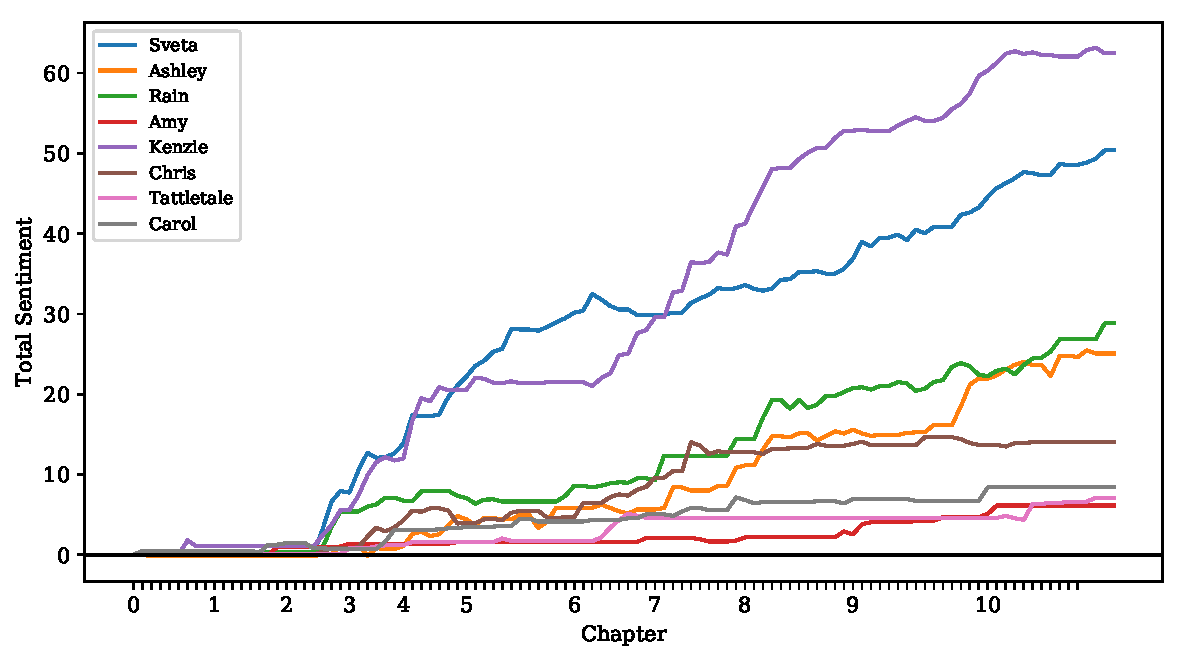
\includegraphics[width=\textwidth]{Full Graphs/total_sent_scores.pdf}
\caption{Cumulative Sentiment over Time Using the TextBlob Classifier}
\label{sent_compare_1}
\end{subfigure}
~
\begin{subfigure}[t]{0.485\textwidth}
\centering
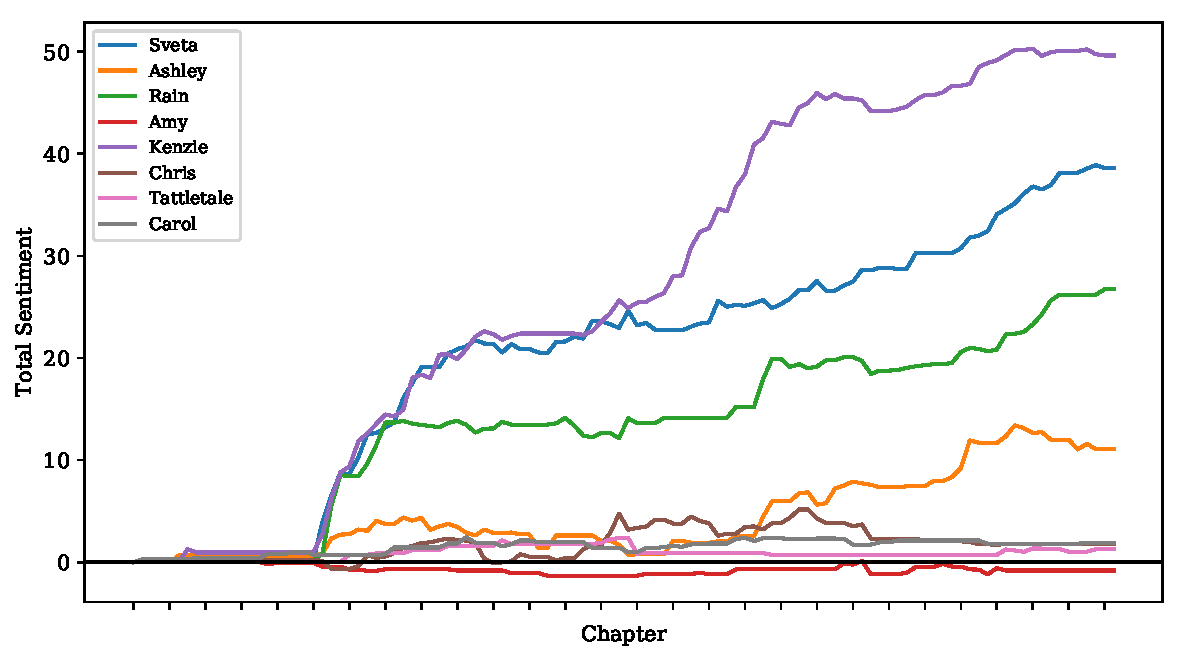
\includegraphics[width=\textwidth]{Full Graphs v2/total_sent_scores.pdf}
\caption{Cumulative Sentiment over Time Using NLTK's VADER Classifier}
\label{sent_compare_2}
\end{subfigure}
\caption{Comparison of the Cumulative Sentiment Total Given by Two Different Classifiers}
\label{sent_anal_comparison}
\end{figure}

\noindent
The next question is how to best display the individual, chapter-by-chapter averaged sentiments. As can be seen from Fig.~\ref{smooth_compare_1}, leaving the results in raw form leads to very noisy and illegible graph. Thus we can smooth out the results by using previous values to influence the current value. The first and simplest way to do this is to just compute a rolling average. In Fig.~\ref{smooth_compare_2} this was done using a window size of 5, meaning that the fifth data point would be displayed as the average of datapoints 1-5. Earlier points were just interpolated from the first and fifth points. This gives a somewhat boxy but certainly more legible result. The second smoothing method we can try is \emph{exponential smoothing}. This is given by the recursive formula
\begin{align*}
s_t = \alpha x_t + (1-\alpha)s_{t-1},
\end{align*}
where $\alpha$ is an input smoothing factor ($\alpha=0.5$ was used here) and $t$ just keeps track of which datapoint we're talking about. Because the value of $s_{t-1}$ is influenced by the previous smoothed points, it's easy to work out this formula's relation to an exponential, though that's neither here nor there. Looking at Fig.~\ref{smooth_compare_3}, we see that this doesn't help much, do the large number of datapoints, the very noisy nature of the data, and the limited window that exponential smoothing looks at (though I suppose a very low $\alpha$ value may help; I haven't bothered to check yet). As such, I will use the rolling average method for the rest of this little investigation.  

\begin{figure}[H]
\centering
\begin{subfigure}[t]{0.485\textwidth}
\centering
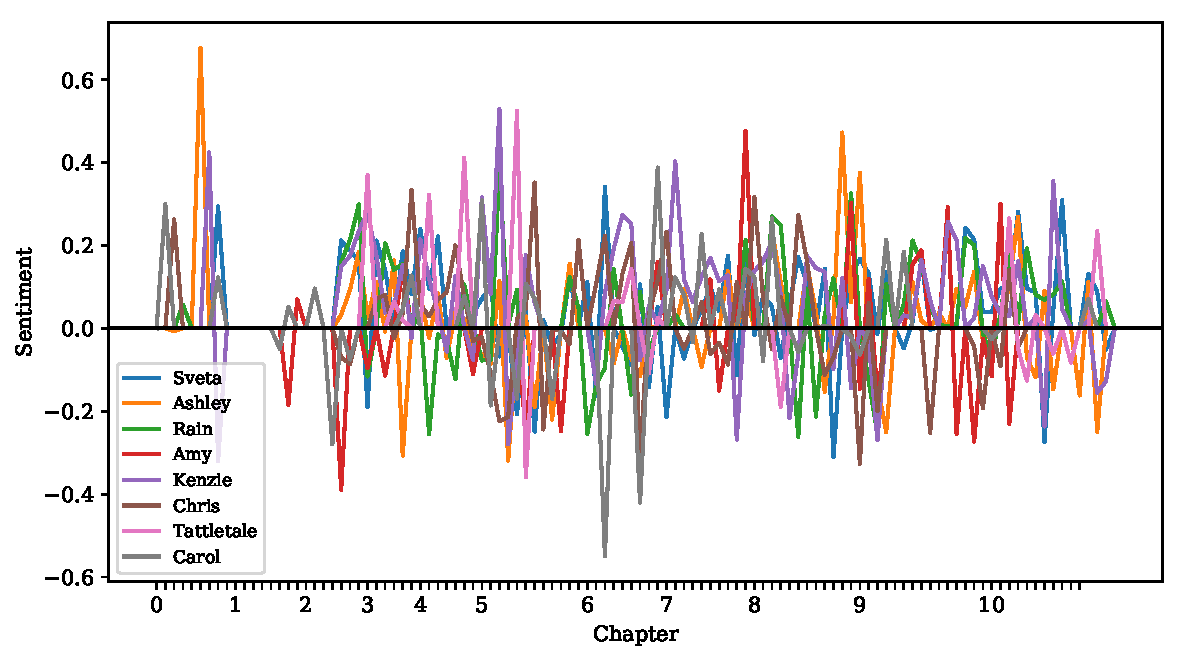
\includegraphics[width=\textwidth]{Full Graphs v2/ind_sent_scores.pdf}
\caption{Individual Chapter Normed Sentiment Scores}
\label{smooth_compare_1}
\end{subfigure}

\begin{subfigure}[t]{0.485\textwidth}
\centering
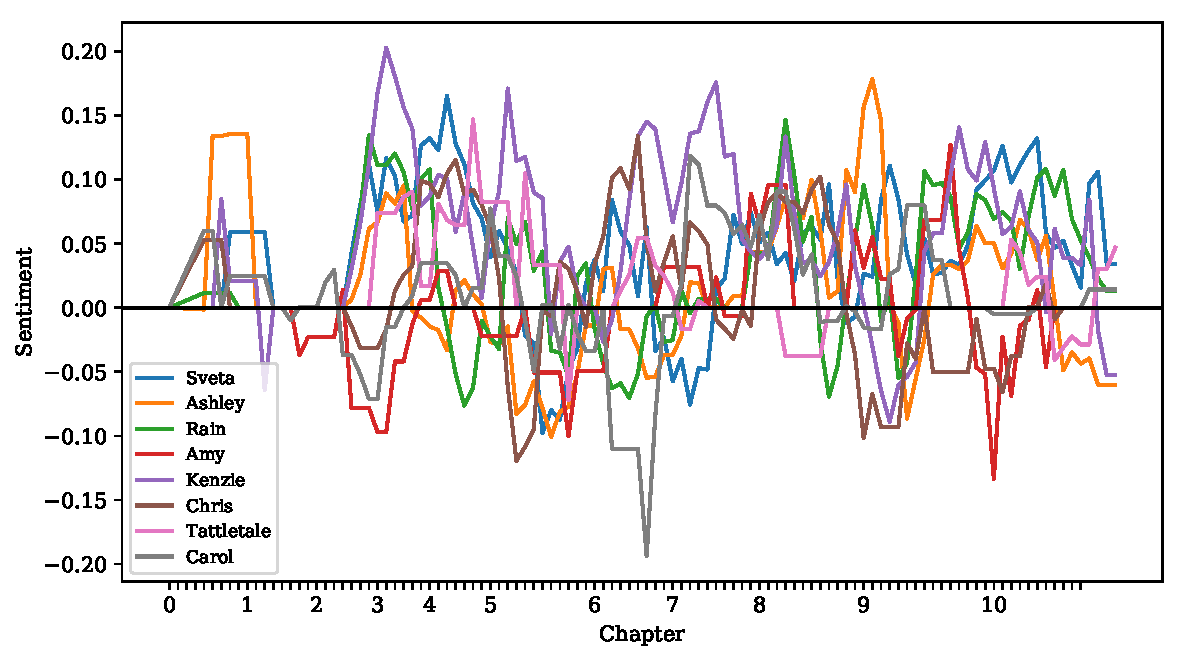
\includegraphics[width=\textwidth]{Full Graphs v2/mean_smoothed_sent_scores.pdf}
\caption{Rolling Average Normed Sentiment Scores}
\label{smooth_compare_2}
\end{subfigure}
~
\begin{subfigure}[t]{0.485\textwidth}
\centering
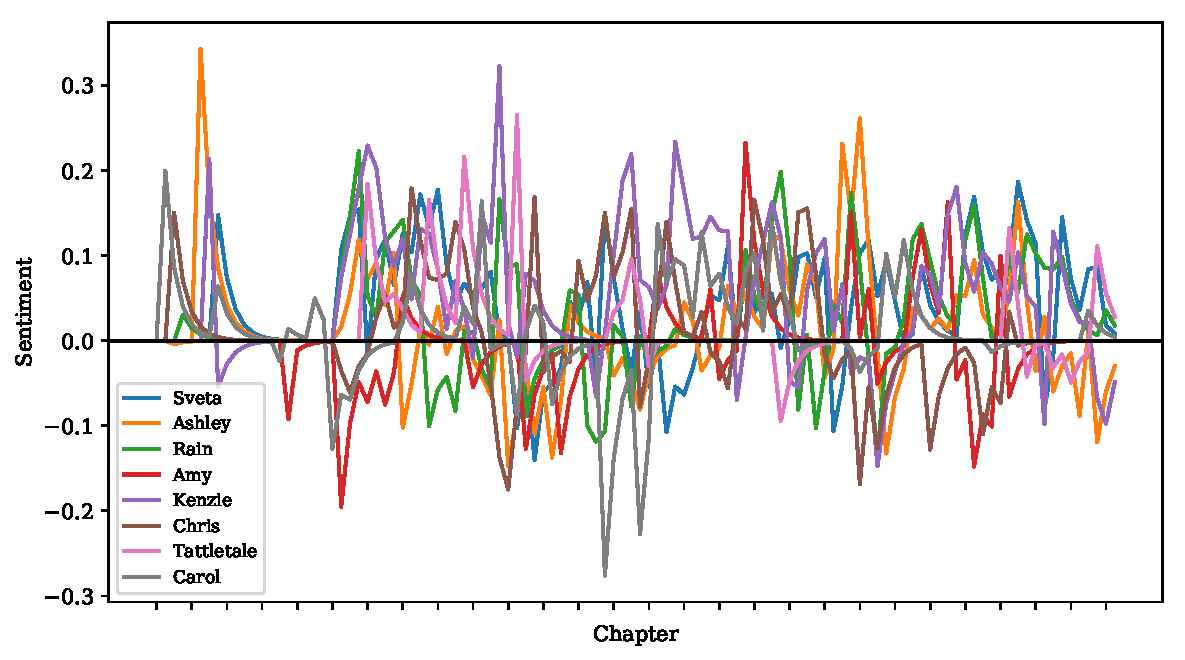
\includegraphics[width=\textwidth]{Full Graphs v2/exp_smooth_sent_scores.pdf}
\caption{Exponentially Smoothed Sentiment Scores}
\label{smooth_compare_3}
\end{subfigure}
\label{smoothing_comparison}
\caption{Comparison of Different Smoothing Methods for the Individual Chapter Scores}
\end{figure}

\noindent
With the questions of methodology settled, let's next look at the results of smaller groups of characters, so that we can look at things more closely. We'll start by looking at the scores for Ashley, Rain, and Chris, members of Victoria's team, Breakthrough, whom she has somewhat mixed opinions on. Looking at the total scores first (Fig.~\ref{arc_total}), we see that Rain was generally viewed in a positive light, while both Chris and Ashley were viewed in a more mixed light, with the sentiments around Ashley ending up being more positive, while those around Chris ended up being neutral to even negative, fitting, given his recent traitorous turn (though this analysis only covers up to chapter 10.11). Looking at the more granular plot in Fig.~\ref{arc_mean}, we can get a better sense of how the sentiment evolved over time. All three had positive spikes early on, as those chapters were actually Glow-Worm, which especially explains Ashley's likely Kenzie induced spike. For Rain, we see him dip during the Fallen raid arc, where his dark past is revealed and he has to go through A LOT of shit, and then trend positive for the rest of the story. Similarly, we see Ashley get described with mixed to negative sentiments early on, before Victoria figures her out and before Ashley mellows out. We also see a dip later on, likely due to the introduction of Ashley's clone sister, `Ashley Black/Slashley'. Finally, Chris bounces all over the place for most of the story, fitting for his moniker of `Cryptid'. However, at the end, when he decides to leave the team and join Amy on Earth Shin, we see the sentiment stay relatively negative. 

\begin{figure}[H]
\centering
\begin{subfigure}[t]{0.75\textwidth}
\centering
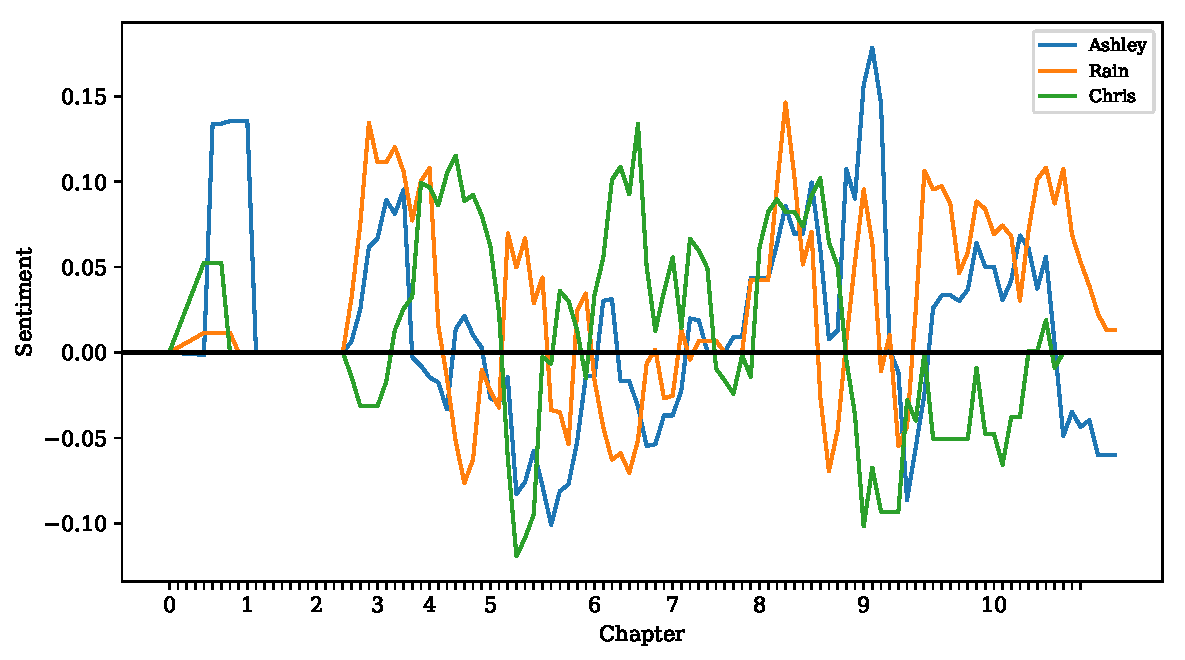
\includegraphics[width=\textwidth]{ARC Graphs v2/mean_smoothed_sent_scores.pdf}
\caption{Mean Smoothed Chapter Scores for Ashley/Rain/Chris}
\label{arc_mean}
\end{subfigure}
~
\begin{subfigure}[t]{0.75\textwidth}
\centering
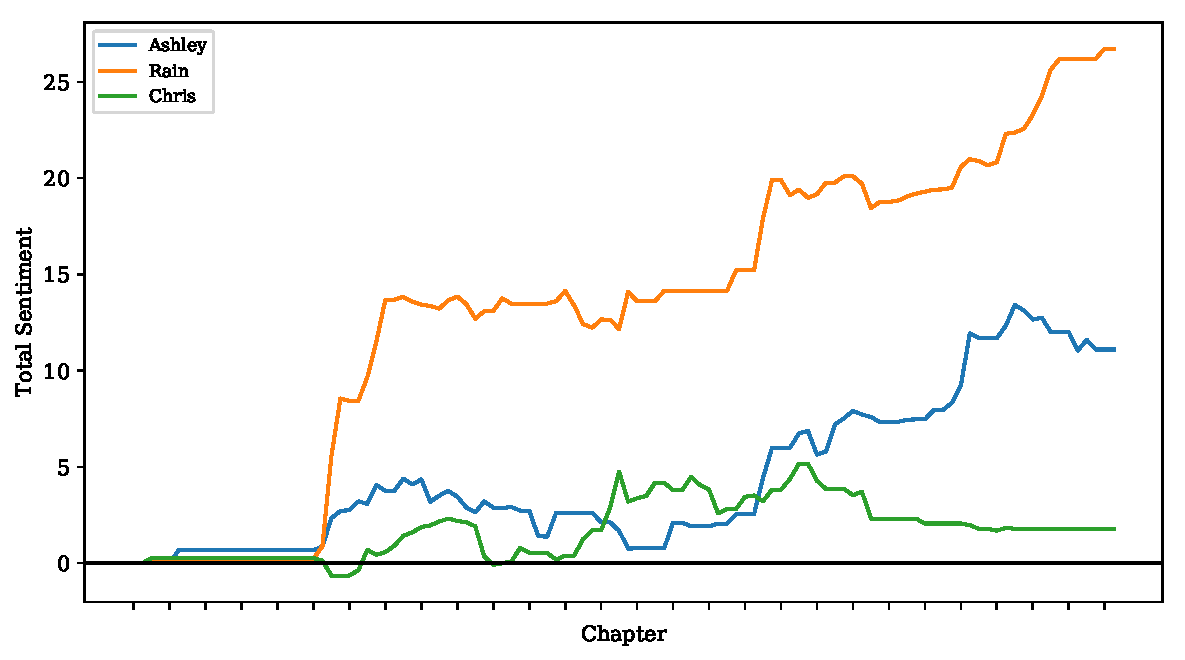
\includegraphics[width=\textwidth]{ARC Graphs v2/total_sent_scores.pdf}
\caption{Cumulative Sentiment Scores for Ashley/Rain/Chris}
\label{arc_total}
\end{subfigure}
\label{arc_graphs}
\caption{Sentiment Scores for Ashley/Rain/Chris}
\end{figure}

\noindent
Next, we'll look at the two members of Breakthrough who Victoria holds in the most positive light; the kid tinker Kenzie and the best friend/`team mom' Sveta. Looking at Fig.~\ref{fem_tot}, we see that both are viewed in an overwhelmingly positive light. Looking at Fig~\ref{fem_mean}, we see that Kenzie is almost never described negatively, with only three real exceptions; early negative mentions during Glow-Worm, likely from Chris and/or Mayday, random points during the midpoint of the story, and when she was brainwashed by Goddess during the prison incident. Looking at Sveta's graph we see similar dips during the story's midsection; looking closer, these seem to be during the end part of the tense Fallen incident and during Breakthrough's rough TV appearance, where the hosts (and not the main character, Victoria) spoke negatively towards pretty much the entire team.

\begin{figure}[H]
\centering
\begin{subfigure}[t]{0.75\textwidth}
\centering
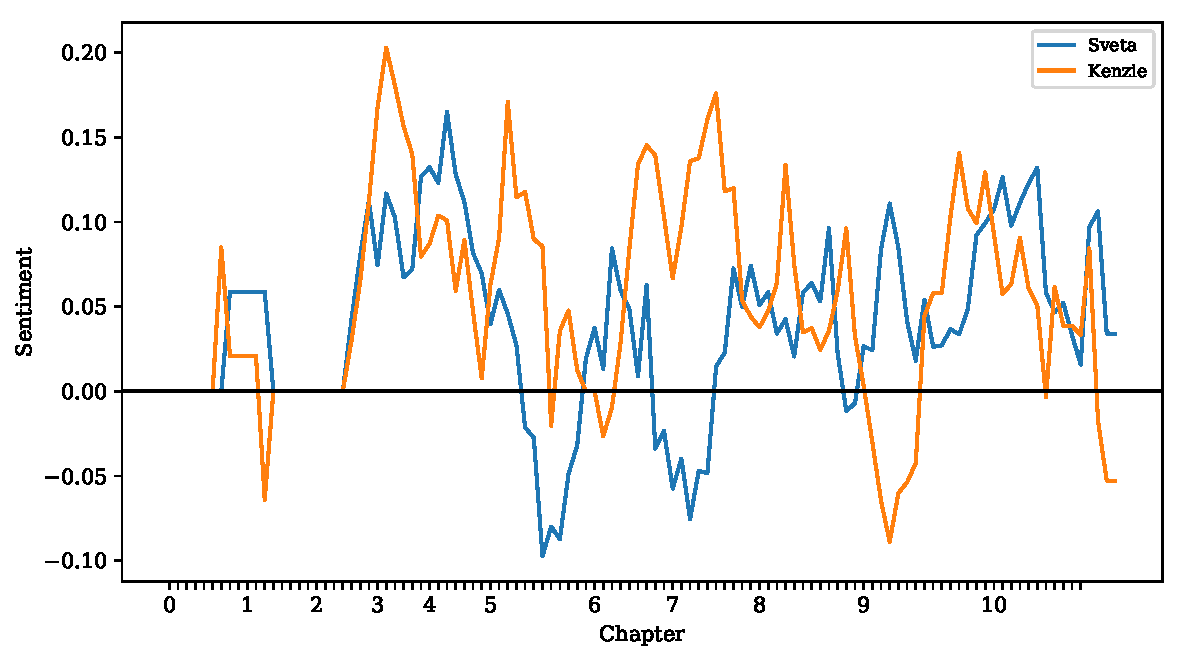
\includegraphics[width=\textwidth]{Fem Graphs v2/mean_smoothed_sent_scores.pdf}
\caption{Mean Smoothed Chapter Scores for Sveta/Kenzie}
\label{fem_mean}
\end{subfigure}
~
\begin{subfigure}[t]{0.75\textwidth}
\centering
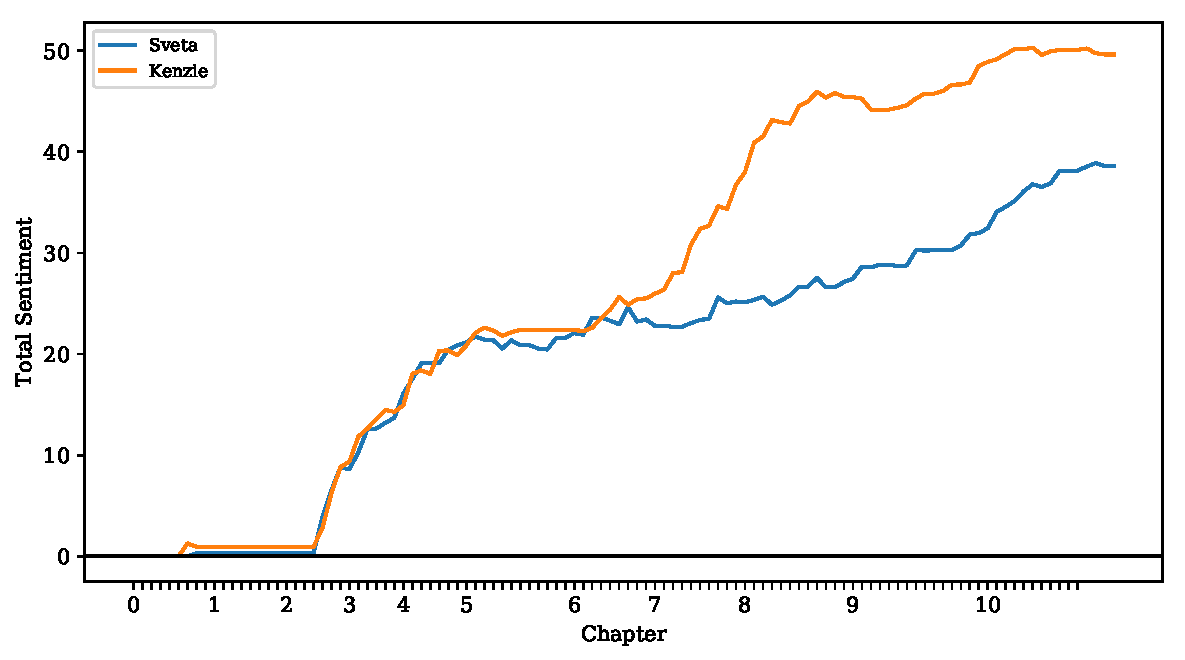
\includegraphics[width=\textwidth]{Fem Graphs v2/total_sent_scores.pdf}
\caption{Cumulative Sentiment Scores for Sveta/Kenzie}
\label{fem_tot}
\end{subfigure}
\caption{Sentiment Scores for Sveta/Kenzie}
\label{fem_graphs}
\end{figure}

\noindent
Finally, we move on to a trio of morally grey but antagonistic characters (especially in the eyes of our main character); the villainous mastermind Tattletale, Victoria's mother Carol (who needs to `Mom the fuck up'), and the source of most of Victoria's nightmares, her sister Amy. It's safe to say that these are the main character's three least favorite people, while also not being clearly evil or villains (despite this being Tattletale's technical position).  As side characters, we expect to see less change among these three than the other five, as they aren't usually focused on, which is easy to given the shape and magnitude of the sentiment totals, as shown in Fig.~\ref{aux_total}. Unsurprisingly, Amy's sentiment is almost always below water, with the only exception being the chapter (8.12) where Victoria defends her during the national television incident (the other spike is due to others discussing Amy or Sveta referring to herself as a `kid sister'). With regards to Tattletale, we see that sentiments regarding her are actually fairly positive (best friends incoming?), though we do see a sharp positive increase followed by a precipitous drop near the middle of the graph; this is in the aftermath of the Fallen raid where first Tattletale offers to help our heroes, with the fall being when they actually talk to her (and roast her a bit) in person. We also see that Carol sits a bit above water too, partly due to Victoria's mixed but somewhat positive feelings towards her and the positive views held by other characters, namely Natalie. The large negative spikes, seen in Fig.~\ref{aux_mean}, are largely spurious, due to one off hand mention and the discussion of other mothers. This is the problem with detecting Carol by looking for the terms mom \& mother; the terms are quite ambiguous. 

\begin{figure}[H]
\centering
\begin{subfigure}[t]{0.75\textwidth}
\centering
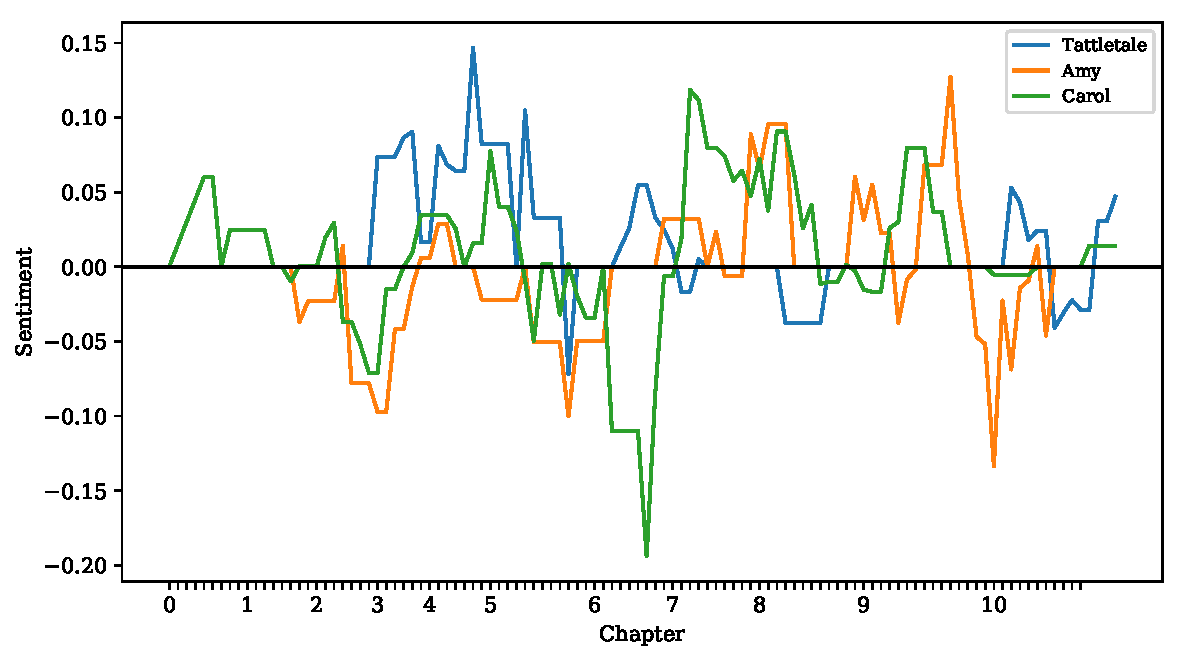
\includegraphics[width=\textwidth]{Aux Graphs v2/mean_smoothed_sent_scores.pdf}
\caption{Mean Smoothed Chapter Scores for Amy/Carol/Tattletale}
\label{aux_mean}
\end{subfigure}
~
\begin{subfigure}[t]{0.75\textwidth}
\centering
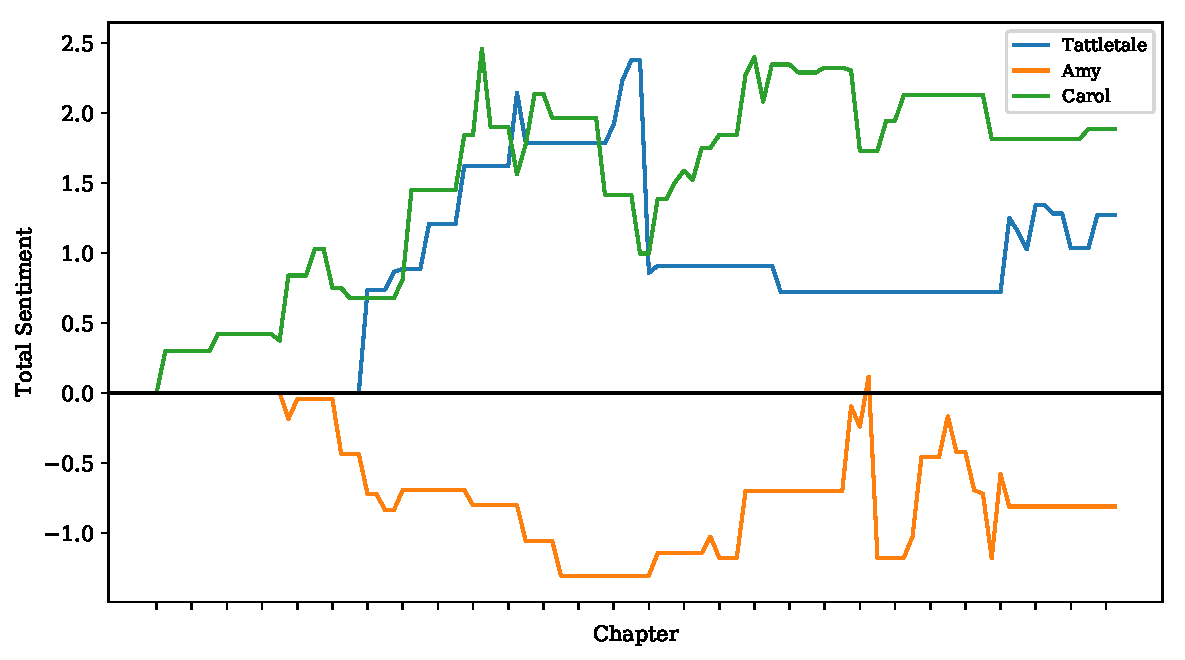
\includegraphics[width=\textwidth]{Aux Graphs v2/total_sent_scores.pdf}
\caption{Cumulative Sentiment Scores for Amy/Carol/Tattletale}
\label{aux_total}
\end{subfigure}
\caption{Sentiment Scores for Amy/Carol/Tattletale}
\label{aux_graphs}
\end{figure}

\section{Conclusion}
\noindent
So what was the point of all of this? Well really, it was just to play around with NLP and sentiment analysis, to get a feel for some of what they can do and bit of how they work. We've definitely run into some limitations of the commonly available methods and of my own knowledge and abilities. One obvious issue is the ambiguity of the text. In general, the idea was to get the point of view character's perspective, but I've made no real effort to make sure only her thoughts and words were analyzed. Furthermore, Amy \& Carol are often referred to by general nouns that may refer to others as well. Additionally, many references may be made using pronouns (he, him, she, her, etc.), and I have yet to really look into whether or not there is an easy way to automatically detect what a pronoun is pointing at. Outside of correct sentence selection, the sentiment analyzers are going to be far from perfect; a quick \href{https://www.quora.com/What-is-the-accepted-accuracy-of-sentiment-analysis}{Quora search} shows that even custom models top out at 70 - 80 \% accuracy and I'm using models trained on different text sources, thought the more general construction methodology for the VADER classifier matches well with its qualitatively superior results. For fun, I may try to create my own simple Naive Bayes classifier to see how the results compare, but I doubt it will improve things on this front. And of course, there are always the usual odds and ends; cleaning up code, prettying graphs and their labels, etc. Regardless of all this, I hope whomever is reading this enjoyed it in some capacity, either by learning something or just enjoying some oscillating lines. 


\end{document}


